\subsection{PCA projection}

The data is now projected onto the two principal component axes mentioned above:

\begin{figure}[H]
    \centering
    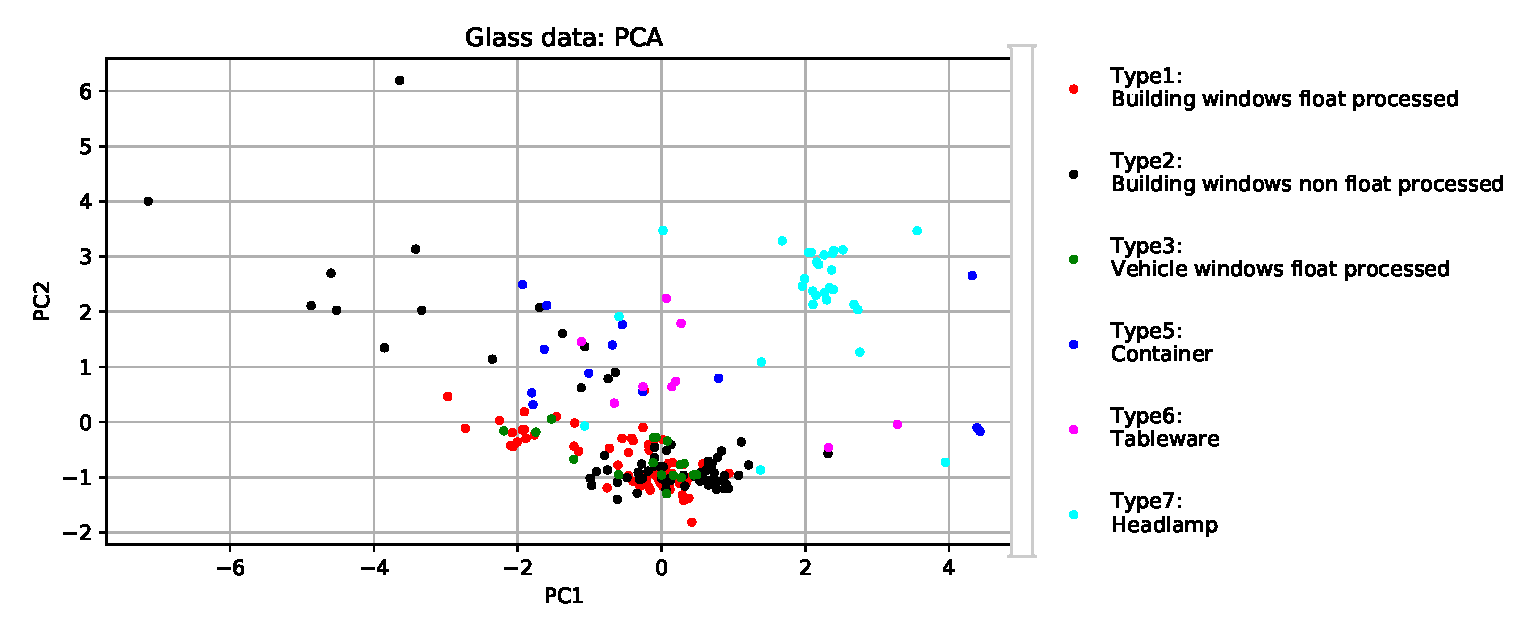
\includegraphics[width=1\linewidth]{fig/PCAStdNormed.eps}
    \caption{Data projection onto first two principal components (eigenvectors). The data set is normalized with respect to standard deviation, and centered around origo. The type "Vehicle windows non float processed" is not present, since no observations of this type appears in the dataset.}
    \label{fig:PCAplot}
\end{figure}

Looking at fig \ref{fig:PCAplot}, a good portion of the data is spread out, but still with a grouping of the top three types (in order by the legend) around origo. From this visualization, it suggests that the type "headlamp" would be classified with the highest accuracy. Funnily enough, it seems that the accuracy of the classifications might end up being almost inversely proportional to the ordering of the legends and thereby the indexing of the types. 